% Draft for Earth System Science Data using Copernicus LaTeX package 7.16.
% Numbers reflect docs/data_processing_record.md as of 2026-09-27.
\documentclass[essd,manuscript]{copernicus}
\usepackage{tikz}
\usetikzlibrary{positioning,arrows.meta,fit}

\begin{document}

\title{A harmonised in situ soil temperature and moisture dataset for Northern Hemisphere soil freeze--thaw studies}

% Confirm author order, affiliations, and corresponding author before submission.
\Author[1]{Hesam}{Salmabadi}
\Author[2]{Alexander}{Roy}
\Author[3]{Aaron}{Berg}

\affil[1]{Affiliation of Hesam Salmabadi to be confirmed}
\affil[2]{Affiliation of Alexander Roy to be confirmed}
\affil[3]{Affiliation of Aaron Berg to be confirmed}

\runningtitle{In situ soil data for freeze--thaw studies}
\runningauthor{Salmabadi et al.}

\received{}
\pubdiscuss{}
\revised{}
\accepted{}
\published{}
\firstpage{1}

\maketitle

\begin{abstract}
Soil freeze--thaw studies need observations across depths, land-cover types,
and spatial scales. We assembled hourly in situ soil temperature and, where
available, volumetric soil moisture from 14 sources into a harmonised collection
of 17,090 sensor records at 2,482 sites in the Northern Hemisphere. The records
span 1991--2026 and contain approximately 808 million valid hourly temperature
values and 133 million valid hourly moisture values. Each sensor has source and
depth metadata, and we link the observations to SoilGrids properties, ten
EASE-Grid 2.0 grids, and land-cover context. We describe source-specific
harmonisation, independent checks of derived metadata, and limitations that
affect use for freeze--thaw applications. The final abstract must cite the
archived, accessible data product and its persistent identifier.
\end{abstract}

\introduction
In situ soil temperature and moisture observations provide reference data for
studies of soil freeze and thaw and for evaluation of gridded products. Their
reuse is complicated by differences in source files, time conventions, sensor
depths, and site metadata. This article documents a harmonised collection of
hourly observations and associated spatial context. The intended product is a
reusable observational resource; freeze--thaw state or transition dates are
not yet part of this dataset. A complete introduction and comparison with
existing collections will be developed for submission.

\section{Data and metadata}
The collection contains 17,090 sensor records at 2,482 sites (2,468 distinct
locations) from 14 sources, spanning 1.9--74.7\,$^{\circ}$\,N and 1991--2026
(Table~\ref{tab:sources}). It includes 808.4 million valid hourly soil
temperature values and 133.5 million soil moisture values; 2,934 sensors
measure both at a documented common depth. Each source was processed by a
dedicated importer. Timestamps were converted to UTC, sub-hourly readings were
averaged within each hour, missing hours were left missing, and moisture was
expressed as m\textsuperscript{3}\,m\textsuperscript{-3}. No values were
interpolated or subjected to new anomaly screening; source quality information
was retained where available.

\begin{table}[t]
\caption{Observation sources. Regional and partner records comprise the other
12 sources; counts describe the working collection before a public-release
subset is defined.}
\label{tab:sources}
\centering
\begin{tabular}{lrr}
\hline
Source group & Sensors & Sites \\
\hline
International Soil Moisture Network & 11,774 & 1,728 \\
AmeriFlux BASE & 4,684 & 484 \\
Regional and partner records & 632 & 270 \\
\hline
Total & 17,090 & 2,482 \\
\hline
\end{tabular}
\end{table}

The \texttt{sensor\_id} links each hourly file to four metadata tables
(Fig.~\ref{fig:metadata}). The catalog identifies the source, site, coordinates,
depth or depth interval, original variable and time convention. SoilGrids 2.0
provides depth-matched texture, organic carbon, bulk density, coarse fragments,
soil class and uncertainty at 250\,m resolution \citep{poggio2021}; one of six
standard soil layers is assigned to each sensor. EASE-Grid 2.0 cell identifiers
locate every sensor on Northern Hemisphere and global grids at 6.25--36\,km
\citep{brodzik2012}. ESA CCI 2015 land cover provides the sensor class, six
area-weighted class fractions for each cell, and a representativeness flag for
each sensor--grid pair. That flag requires the sensor class to dominate at
least 70\,\% of the cell, with no more than 5\,\% water or 5\,\% other cover.
The sensor's detailed ESA CCI class (e.g. needleleaved evergreen tree cover,
lichens and mosses) is kept alongside the six merged classes. Because land
cover describes vegetation structure but not climate, it cannot separate
boreal from temperate forest or tundra from prairie grassland; each sensor is
therefore also assigned the biome and ecoregion of RESOLVE Ecoregions 2017
\citep{dinerstein2017}. Seventeen sensors on coasts or lake shores lie just
outside every ecoregion polygon and take the nearest one (at most 2.8\,km
away). Most sensors lie in temperate biomes; 925 are in boreal forest and 847 in
tundra (Table~\ref{tab:biome-soil}). Biomes describe potential natural
vegetation, so cropland is the most common cover in the temperate broadleaf
and grassland biomes. Boreal and tundra sites have the most organic-rich and
least dense soils (median SOC 72 and 99\,g\,kg$^{-1}$).

\begin{table*}[t]
\caption{Sites and sensors by RESOLVE Ecoregions 2017 biome \citep{dinerstein2017}, with the two most common ESA CCI land-cover classes of the sensors' 300\,m pixels and SoilGrids 2.0 properties of the layer matched to each sensor's depth, as median (10th--90th percentile). Topsoil: $2.5 < z < 7.5$\,cm or a 0--5\,cm integrating probe.}
\label{tab:biome-soil}
\centering
\scriptsize
\begin{tabular}{p{3.2cm}rrrp{4.2cm}llll}
\tophline
Biome & Sites & Sensors & Topsoil & Main land cover (ESA CCI) & Clay (\%) & Sand (\%) & SOC (g\,kg$^{-1}$) & Bulk density (g\,cm$^{-3}$) \\
\middlehline
Temperate Broadleaf \& Mixed Forests & 544 & 4,048 & 861 & cropland, herbaceous 32\%; grassland 20\% & 21 (7--35) & 42 (13--74) & 29 (4--95) & 1.34 (1.04--1.63) \\
Temperate Grasslands, Savannas \& Shrublands & 446 & 3,914 & 841 & cropland, herbaceous 41\%; grassland 34\% & 30 (15--39) & 32 (8--65) & 12 (3--43) & 1.53 (1.30--1.69) \\
Temperate Conifer Forests & 468 & 3,248 & 869 & tree, needleleaved evergreen 67\%; tree, broadleaved deciduous 10\% & 17 (8--29) & 45 (30--66) & 22 (7--108) & 1.26 (0.99--1.51) \\
Deserts \& Xeric Shrublands & 415 & 2,578 & 661 & shrubland 42\%; cropland, rainfed 14\% & 20 (14--30) & 45 (28--66) & 10 (2--24) & 1.46 (1.30--1.56) \\
Boreal Forests/Taiga & 182 & 925 & 209 & tree, needleleaved evergreen, closed 30\%; tree, needleleaved evergreen 18\% & 13 (7--31) & 43 (20--68) & 72 (21--224) & 1.06 (0.63--1.33) \\
Tundra & 169 & 847 & 158 & lichens and mosses 22\%; shrubland 15\% & 15 (9--27) & 40 (26--52) & 99 (39--310) & 0.99 (0.42--1.27) \\
Montane Grasslands \& Shrublands & 117 & 555 & 131 & grassland 93\%; sparse vegetation 3\% & 16 (12--22) & 58 (31--62) & 29 (12--64) & 1.26 (1.12--1.38) \\
Mediterranean Forests, Woodlands \& Scrub & 89 & 485 & 109 & grassland 27\%; cropland, rainfed 19\% & 26 (14--32) & 37 (26--66) & 21 (5--59) & 1.43 (1.27--1.60) \\
Tropical \& Subtropical Dry Broadleaf Forests & 11 & 187 & 36 & cropland, rainfed 35\%; grassland 26\% & 39 (34--51) & 27 (18--38) & 16 (4--52) & 1.47 (1.18--1.83) \\
Tropical \& Subtropical Grasslands, Savannas \& Shrublands & 13 & 134 & 31 & cropland, rainfed 53\%; grassland 13\% & 30 (17--37) & 43 (18--62) & 11 (3--40) & 1.59 (1.27--1.84) \\
Tropical \& Subtropical Moist Broadleaf Forests & 19 & 104 & 21 & tree, broadleaved evergreen 52\%; cropland, rainfed 17\% & 38 (33--62) & 26 (16--40) & 25 (6--64) & 1.31 (1.00--1.47) \\
Flooded Grasslands \& Savannas & 5 & 39 & 11 & shrub or herbaceous, flooded 74\%; cropland, rainfed 26\% & 27 (24--38) & 27 (12--34) & 119 (44--148) & 0.98 (0.76--1.12) \\
Tropical \& Subtropical Coniferous Forests & 1 & 21 & 3 & tree, needleleaved evergreen 100\% & 8 (8--9) & 66 (66--67) & 32 (6--89) & 1.14 (1.14--1.33) \\
Mangroves & 3 & 5 & 1 & tree, flooded, saline water 60\%; water 40\% & 27 (26--29) & 36 (20--42) & 132 (108--212) & 0.49 (0.25--0.57) \\
\bottomhline
\end{tabular}
\end{table*}


\begin{figure}[t]
\centering
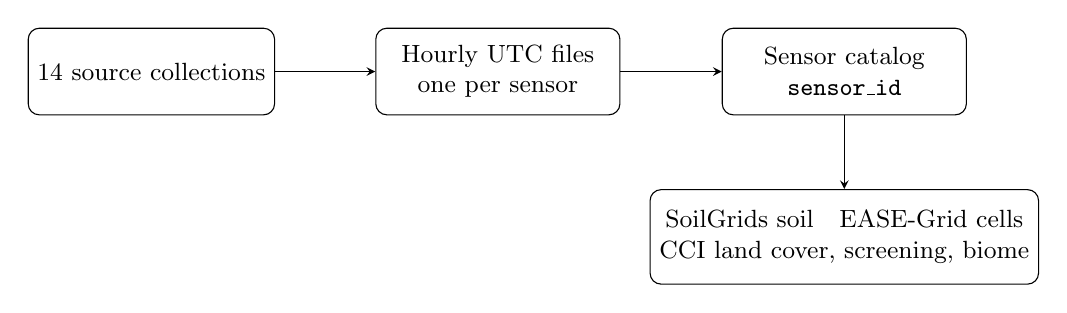
\begin{tikzpicture}[>=stealth, every node/.style={font=\small}]
\node[draw, rounded corners, align=center, minimum width=3.1cm, minimum height=1.1cm] (src) at (0,0) {14 source collections};
\node[draw, rounded corners, align=center, minimum width=3.1cm, minimum height=1.1cm] (hour) at (4.4,0) {Hourly UTC files\\one per sensor};
\node[draw, rounded corners, align=center, minimum width=3.1cm, minimum height=1.1cm] (cat) at (8.8,0) {Sensor catalog\\\texttt{sensor\_id}};
\node[draw, rounded corners, align=center, minimum width=4.3cm, minimum height=1.2cm] (anc) at (8.8,-2.1) {SoilGrids soil\quad EASE-Grid cells\\CCI land cover, screening, biome};
\draw[->] (src) -- (hour);
\draw[->] (hour) -- (cat);
\draw[->] (cat) -- (anc);
\end{tikzpicture}
\caption{Observation files and derived metadata are joined by the unique sensor identifier.}
\label{fig:metadata}
\end{figure}

\section{Soil freeze--thaw state}
\label{sec:state}
Hourly probabilities of thawed, transitional and frozen soil and yearly freeze
dates are derived for topsoil sensors in three steps (Fig.~\ref{fig:workflow}):
freezing thresholds are fitted where soil moisture or permittivity is measured
(Sect.~\ref{sec:state-permittivity}), borrowed where only soil temperature is
available or no fit was accepted (Sect.~\ref{sec:state-temperature}), and
applied hour by hour with their uncertainty (Sect.~\ref{sec:state-hourly}).

\begin{figure*}[t]
\centering
\resizebox{\textwidth}{!}{% Workflow of the freeze--thaw state (Sect. 3). Included by main.tex.
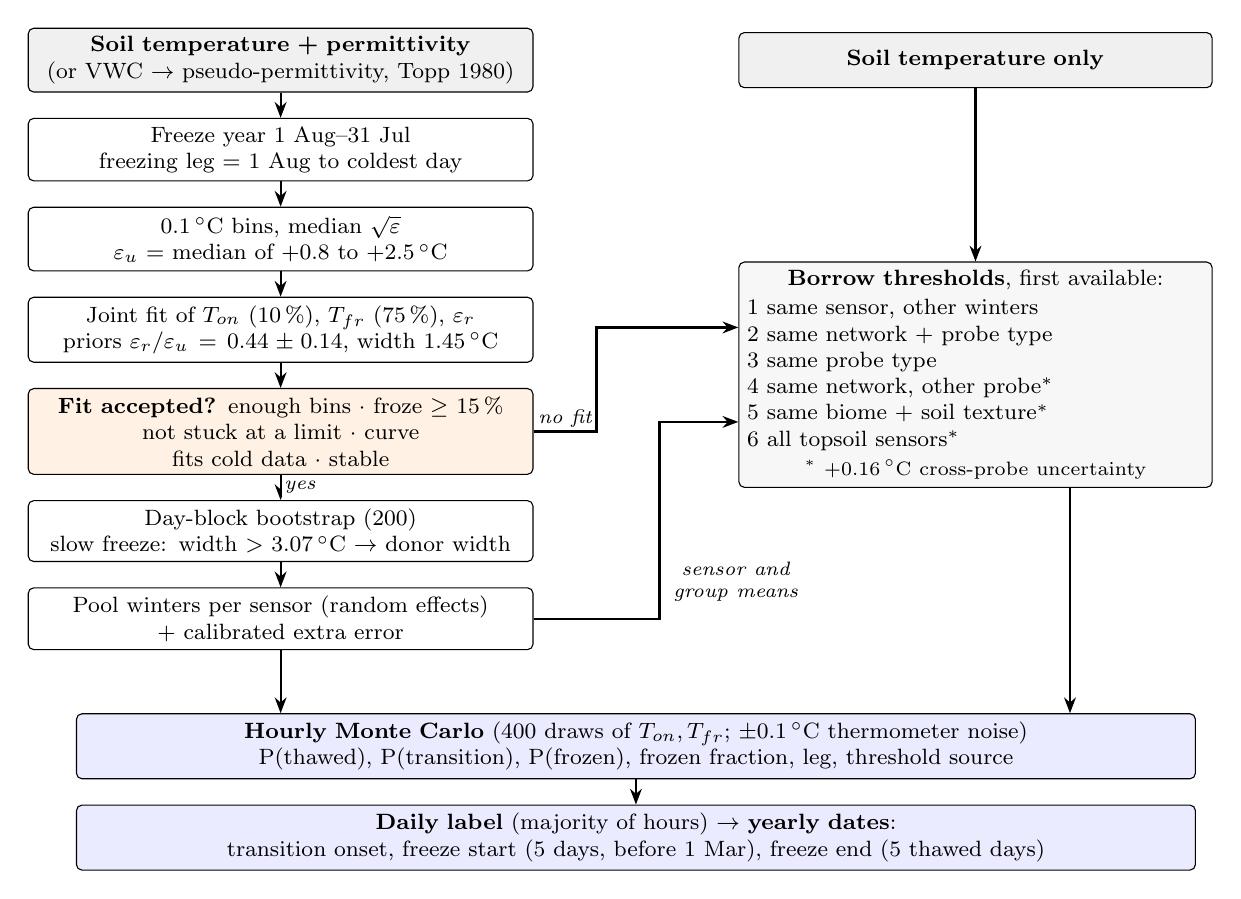
\begin{tikzpicture}[
  font=\footnotesize, node distance=3.2mm and 5mm,
  box/.style={draw, rounded corners=2pt, align=center, text width=#1, inner sep=3pt, minimum height=7mm},
  box/.default=62mm,
  inbox/.style={box=#1, fill=black!6},
  out/.style={box=#1, fill=blue!8},
  choice/.style={box=#1, fill=orange!10},
  arr/.style={-{Stealth[length=2mm]}, thick},
  lab/.style={font=\scriptsize\itshape, midway, fill=white, inner sep=1pt}]
% --- left column: sensors with moisture or permittivity
\node[inbox=62mm] (in1) {\textbf{Soil temperature + permittivity}\\(or VWC $\to$ pseudo-permittivity, Topp 1980)};
\node[box, below=of in1] (leg) {Freeze year 1 Aug--31 Jul\\freezing leg = 1 Aug to coldest day};
\node[box, below=of leg] (bin) {0.1\,$^{\circ}$C bins, median $\sqrt{\varepsilon}$\\$\varepsilon_u$ = median of $+0.8$ to $+2.5$\,$^{\circ}$C};
\node[box, below=of bin] (fit) {Joint fit of $T_{on}$ (10\,\%), $T_{fr}$ (75\,\%), $\varepsilon_r$\\priors $\varepsilon_r/\varepsilon_u = 0.44 \pm 0.14$, width 1.45\,$^{\circ}$C};
\node[choice, below=of fit] (acc) {\textbf{Fit accepted?} enough bins $\cdot$ froze $\ge$ 15\,\%\\not stuck at a limit $\cdot$ curve fits cold data $\cdot$ stable};
\node[box, below=of acc] (boot) {Day-block bootstrap (200)\\slow freeze: width $>$ 3.07\,$^{\circ}$C $\to$ donor width};
\node[box, below=of boot] (pool) {Pool winters per sensor (random effects)\\+ calibrated extra error};
% --- right column: temperature only / no fit
\node[inbox=58mm, right=26mm of in1] (in2) {\textbf{Soil temperature only}};
\node[box=58mm, fill=black!3, below=22mm of in2] (chain) {\textbf{Borrow thresholds}, first available:\\[1pt]
  \raggedright
  1 same sensor, other winters\\
  2 same network + probe type\\
  3 same probe type\\
  4 same network, other probe$^{\ast}$\\
  5 same biome + soil texture$^{\ast}$\\
  6 all topsoil sensors$^{\ast}$\\[1pt]
  {\scriptsize $^{\ast}$ +0.16\,$^{\circ}$C cross-probe uncertainty}};
% --- bottom: shared
\node[out=140mm, below=8mm of pool.south east, anchor=north, xshift=13mm] (mc) {\textbf{Hourly Monte Carlo} (400 draws of $T_{on}, T_{fr}$; $\pm$0.1\,$^{\circ}$C thermometer noise)\\
  P(thawed), P(transition), P(frozen), frozen fraction, leg, threshold source};
\node[out=140mm, below=of mc] (dates) {\textbf{Daily label} (majority of hours) $\to$ \textbf{yearly dates}:\\
  transition onset, freeze start (5 days, before 1 Mar), freeze end (5 thawed days)};
\draw[arr] (in1) -- (leg);
\draw[arr] (leg) -- (bin);
\draw[arr] (bin) -- (fit);
\draw[arr] (fit) -- (acc);
\draw[arr] (acc) -- node[lab, right]{yes} (boot);
\draw[arr] (boot) -- (pool);
\draw[arr] (acc.east) -- node[lab, above]{no fit} ++(8mm,0) |- ([yshift=6mm]chain.west);
\draw[arr] (in2) -- (chain);
\draw[arr] (pool.east) -- ++(16mm,0) coordinate (pv) |- ([yshift=-6mm]chain.west);
\node[font=\scriptsize\itshape, align=center, right=0.5mm of pv, anchor=south west, yshift=1mm] {sensor and\\group means};
\draw[arr] (pool.south) -- (pool.south |- mc.north);
\draw[arr] ([xshift=12mm]chain.south) -- ([xshift=12mm]chain.south |- mc.north);
\draw[arr] (mc) -- (dates);
\end{tikzpicture}
}
\caption{Workflow of the freeze--thaw state. Grey: inputs; orange: acceptance
test of each winter's fit; blue: outputs for every hour and year.}
\label{fig:workflow}
\end{figure*}


\subsection{Sensors with soil moisture or permittivity}
\label{sec:state-permittivity}
For sensors that measure bulk permittivity $\varepsilon$ together with soil
temperature, or volumetric water content converted to (pseudo-)permittivity by
inverting \citet{topp1980}, the freezing of soil water is described by a soil
freezing characteristic curve in permittivity--temperature space
\citep{salmabadi2026}. The method is applied to the topsoil class
($2.5 < z < 7.5$\,cm, plus probes integrating exactly 0--5\,cm; probes
integrating deeper layers such as 0--10\,cm are excluded). Each freeze year (1~August--31~July) is split at the day
of lowest daily-mean soil temperature into a freezing and a thawing leg. The
curve is fitted to the freezing leg only, so that snowmelt infiltration and
thaw hysteresis do not enter the fit. Readings of the freezing leg are grouped
into 0.1\,$^{\circ}$C soil-temperature bins, the resolution of most soil
thermistors, and each bin is summarised by the median of $\sqrt{\varepsilon}$.
Binning weights all temperatures equally, whatever the time the soil spent at
them, and short freeze--thaw episodes near 0\,$^{\circ}$C contribute points to
the same curve instead of being treated as separate events
(Fig.~\ref{fig:binning}).

\begin{figure*}[t]
\centering
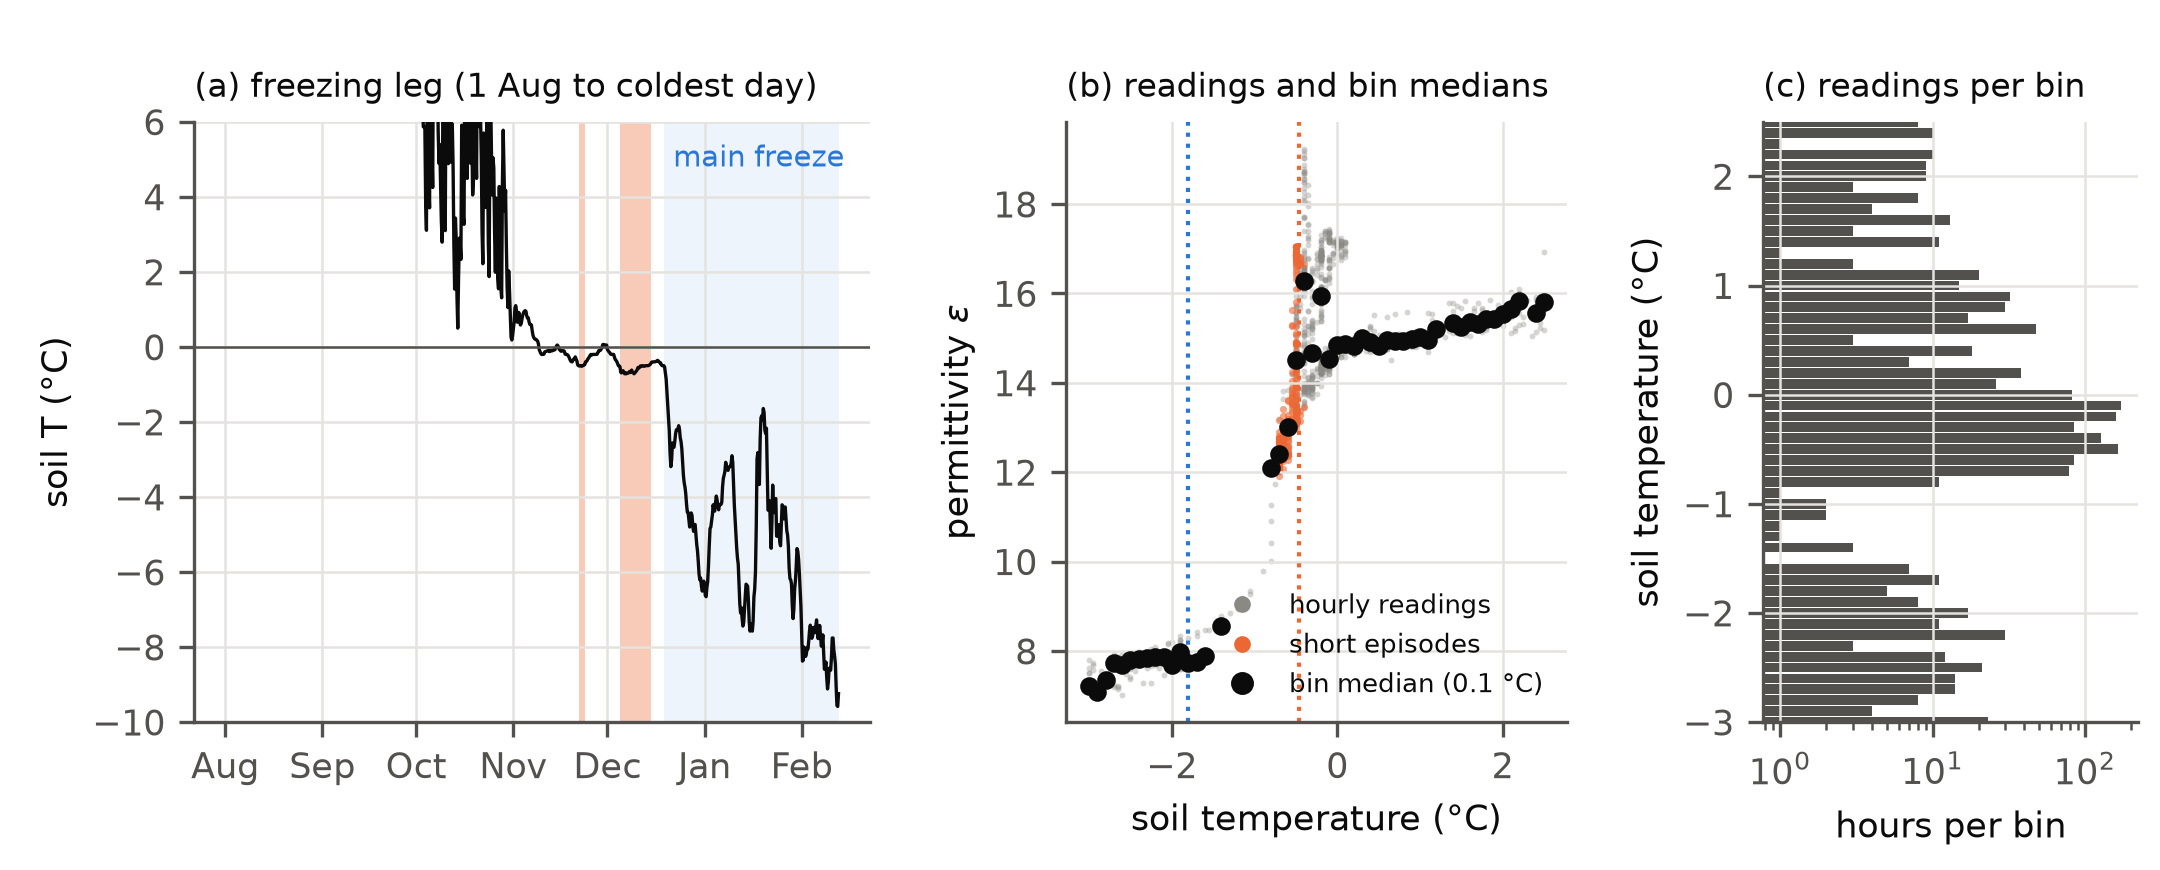
\includegraphics[width=\textwidth]{figures/fig_binning.png}
\caption{Binning of one freezing leg (Kenaston EC02, HydraProbe, 5\,cm, winter
2017--2018). (a) Soil temperature from 1~August to the coldest day; short
episodes below $T_{on}$ before the main freeze are shaded orange. (b) Hourly
readings (grey; episodes in orange) and the median of each 0.1\,$^{\circ}$C bin
(black), with $T_{on}$ and $T_{fr}$ (dotted). (c) Hours per bin: the soil spends
more than 100\,h in single bins near 0\,$^{\circ}$C but only a few hours in the
bins it crosses quickly, and each bin contributes one point to the fit.}
\label{fig:binning}
\end{figure*}

Following \citet{cohen2021}, observations are expressed as a frozen fraction
between an unfrozen level $\varepsilon_u$ and a frozen (residual) level
$\varepsilon_r$,
\begin{equation}
F = \frac{\sqrt{\varepsilon_u} - \sqrt{\varepsilon}}{\sqrt{\varepsilon_u} - \sqrt{\varepsilon_r}},
\label{eq:fraction}
\end{equation}
where the square roots follow a dielectric mixing model with exponent 0.5.
The two levels are obtained as described below (Fig.~\ref{fig:levels}).
The frozen fraction follows the curve of \citet{bai2018},
\begin{equation}
F(T) = 1 - \exp\left[b\,(T - T_f)\right] \quad \text{for } T < T_f, \qquad F(T) = 0 \text{ otherwise},
\label{eq:bai}
\end{equation}
in which the freezing onset $T_f$ is a free parameter to absorb freezing-point
depression and probe offsets \citep{salmabadi2026}. We parametrise
Eq.~(\ref{eq:bai}) directly by the temperatures at which 10\,\% and 75\,\% of the
freezable water is frozen, $T_{on}$ \citep{cohen2021} and $T_{fr}$
\citep{salmabadi2026}, so that
$b = \ln(0.90/0.25)/(T_{on}-T_{fr})$. Soil is thawed above $T_{on}$, frozen
below $T_{fr}$, and in transition between them.

\paragraph{Unfrozen level.} $\varepsilon_u$ is the median permittivity of the
bins between $+0.8$ and $+2.5$\,$^{\circ}$C. The lower limit keeps the window
clear of the freezing onset, which can lie up to about $+0.7$\,$^{\circ}$C
because of thermistor offsets; the upper limit keeps it close to the freezing
point, so that the level reflects the soil moisture just before freezing rather
than the wetter or drier conditions of early autumn. Because each bin counts
once, the median is not dominated by the long periods the soil spends at a
single temperature, and it is robust to a moisture step inside the window
(Fig.~\ref{fig:levels}b, where a change in autumn soil moisture splits the window bins into two
groups).

\paragraph{Frozen level observed.} Once almost all freezable water has
turned to ice, permittivity stops falling as the soil cools further, and the
coldest bins form a flat stretch (Fig.~\ref{fig:levels}a). We used such
winters to learn the typical frozen level and, below, the typical curve width. A winter qualified when (i) its soil
reached $-5$\,$^{\circ}$C, well beyond the typical $T_{fr}$, so that a flat
stretch has room to appear; (ii) the coldest bins formed a flat stretch at
least 0.5\,$^{\circ}$C long; and (iii) permittivity fell by more than 3 units
between the unfrozen and frozen levels, so that the ratio of the two is not
dominated by noise. The flat stretch starts at the coldest bins and extends
towards warmer bins for as long as each bin stays close to the three coldest
ones, where close means within 10\,\% of the total fall of $\sqrt{\varepsilon}$.
In Fig.~\ref{fig:levels}a, $\varepsilon_u = 20.0$ and the three coldest bins
have $\varepsilon \approx 6.7$; the total fall of $\sqrt{\varepsilon}$ is
$4.47-2.56 = 1.91$, so bins within $\pm0.19$ of $\sqrt{6.7}$, that is
$\varepsilon$ between 5.7 and 7.7, belong to the stretch. It runs from
$-6.4$ to $-1.2$\,$^{\circ}$C (43 bins); the bin at $-1.1$\,$^{\circ}$C
($\varepsilon = 7.74$) ends it. The observed $\varepsilon_r$ is the median of
the stretch, 6.9. Across 1,326 qualifying winters at 492 sensors,
$\varepsilon_r/\varepsilon_u$ had a median of 0.44 and a standard deviation of
0.14, and the median width $T_{on}-T_{fr}$ was 1.45\,$^{\circ}$C; these values
are used as priors. For the 1,285 topsoil winters at 467 sensors the ratio
had a median of 0.45 (10th--90th percentile 0.25--0.60;
Fig.~\ref{fig:frozen-fraction}).

\paragraph{Frozen level estimated.} Most winters do not show a plateau: the
soil stays too warm, or it is cold but its permittivity is still falling
(Fig.~\ref{fig:levels}b, c). In production, therefore, $\varepsilon_r$ is not
taken from the plateau rule but estimated for every winter together with
$T_{on}$ and $T_{fr}$, as $\varepsilon_r = f\,\varepsilon_u$, by least squares
on the bins between $-4$ and $+2.5$\,$^{\circ}$C. Residuals are scaled by the
robust scatter of the unfrozen bins, and two penalty terms act as weak priors:
$f \sim \mathcal{N}(0.44, 0.14^2)$ and $\ln(T_{on}-T_{fr}) \sim
\mathcal{N}(\ln 1.45, 0.7^2)$. The fitted frozen level may not exceed the lowest
binned permittivity by more than 5\,\%, since the soil cannot be less frozen
than it was at its coldest. The fit is started from three initial values and the best
solution kept. When cold bins define a plateau, they outweigh the prior and
the fitted level matches the observed one (6.9 in both cases in
Fig.~\ref{fig:levels}a). When the soil is cold but still sinking, the curvature
of the cold bins and the prior together place the level below the lowest bin
(7.9 against a lowest bin of 8.1 in Fig.~\ref{fig:levels}b). When the soil
never freezes completely, the level follows the prior (12.2, i.e.
$0.48\,\varepsilon_u$, in Fig.~\ref{fig:levels}c), and the resulting
uncertainty of $T_{fr}$ is carried forward by the bootstrap and the extra error
terms described below (Fig.~\ref{fig:example-winters}).
A regression of $\varepsilon_r$ on SoilGrids
texture, organic carbon, bulk density and probe type reduced the
leave-one-site-out error only from 1.16 to 1.01 permittivity units and was not
adopted. A winter's fit is accepted only if it passes five checks. (i) Enough data:
the $+0.8$ to $+2.5$\,$^{\circ}$C window contains bins, and at least five bins
lie between $-4$ and $+2.5$\,$^{\circ}$C. (ii) The soil froze noticeably: the
lowest permittivity reached (median of three neighbouring cold bins) covers at
least 15\,\% of the way, on the $\sqrt{\varepsilon}$ scale, from $\varepsilon_u$
to the expected frozen level $0.44\,\varepsilon_u$; otherwise there is no curve
to fit. (iii) No parameter rests on its limit ($T_{on}$ between $-2$ and
$+1.5$\,$^{\circ}$C, width below 7.5\,$^{\circ}$C, $\varepsilon_r/\varepsilon_u$
above 0.03), because a solution held by a limit is set by the limit rather
than by the data. (iv) The curve matches the cold data: the root-mean-square
difference between curve and bins colder than $T_{on}+0.3$\,$^{\circ}$C is at
most 30\,\% of the total fall $\sqrt{\varepsilon_u}-\sqrt{\varepsilon_r}$. (v)
The result is stable: at least half of the bootstrap replicates described
below give an accepted fit (checks i--iii). In the topsoil class, 4,846 of
11,884 sensor-winters with moisture data passed; 3,812 failed check (i), 2,472
check (ii), 352 check (iii), 226 check (iv) and 176 check (v). Most failures
are winters that never cooled near 0\,$^{\circ}$C or barely froze, and these
borrow thresholds like temperature-only sensors
(Sect.~\ref{sec:state-temperature}).

\paragraph{Slow freezes.} In some winters the fitted curve is very wide: the
permittivity falls slowly over several degrees, and $T_{fr}$ lies far below
$T_{on}$. We treat such curves as unreliable, whatever the soil. As reference
we use the fitted winters whose frozen level is seen in the data by the
flat-stretch rule above, because only there is the whole curve measured
(Fig.~\ref{fig:widths}). Their median width was 1.51\,$^{\circ}$C, consistent
with the width prior, and their 90th percentile 3.07\,$^{\circ}$C. Winters
wider than that (339 of 4,846 fitted topsoil winters, 7.0\,\%) keep their
$T_{on}$, but $T_{fr}$ is replaced by $T_{on}$ minus the median width of
reference winters that are not wide themselves, taken from the first of these
groups with at least three such winters: the same sensor, the same network and
probe type, the same probe type, the same biome and soil texture, or all
topsoil winters. The spread of the borrowed widths is added to the uncertainty
of $T_{fr}$. Wide curves are more common in dry soils (16\,\% of winters with
$\varepsilon_u \le 6$ against 2\,\% with $\varepsilon_u > 20$;
Fig.~\ref{fig:widths}b) but are replaced there as well.

Uncertainty is estimated with a bootstrap of 200 replicates that resample whole
days with replacement and redraw the prior centres, repeating the binning and
the fit. $T_{on}$ and $T_{fr}$ are the replicate medians and their spread the
fitting uncertainty; to reach nominal 95\,\% coverage on a synthetic benchmark
with known thresholds, 0.1\,$^{\circ}$C is added to $T_{on}$ and 0.2, 0.5 or
1.0\,$^{\circ}$C to $T_{fr}$ when the soil went at least 1\,$^{\circ}$C below,
less than 1\,$^{\circ}$C below, or never below $T_{fr}$.

\begin{figure*}[t]
\centering
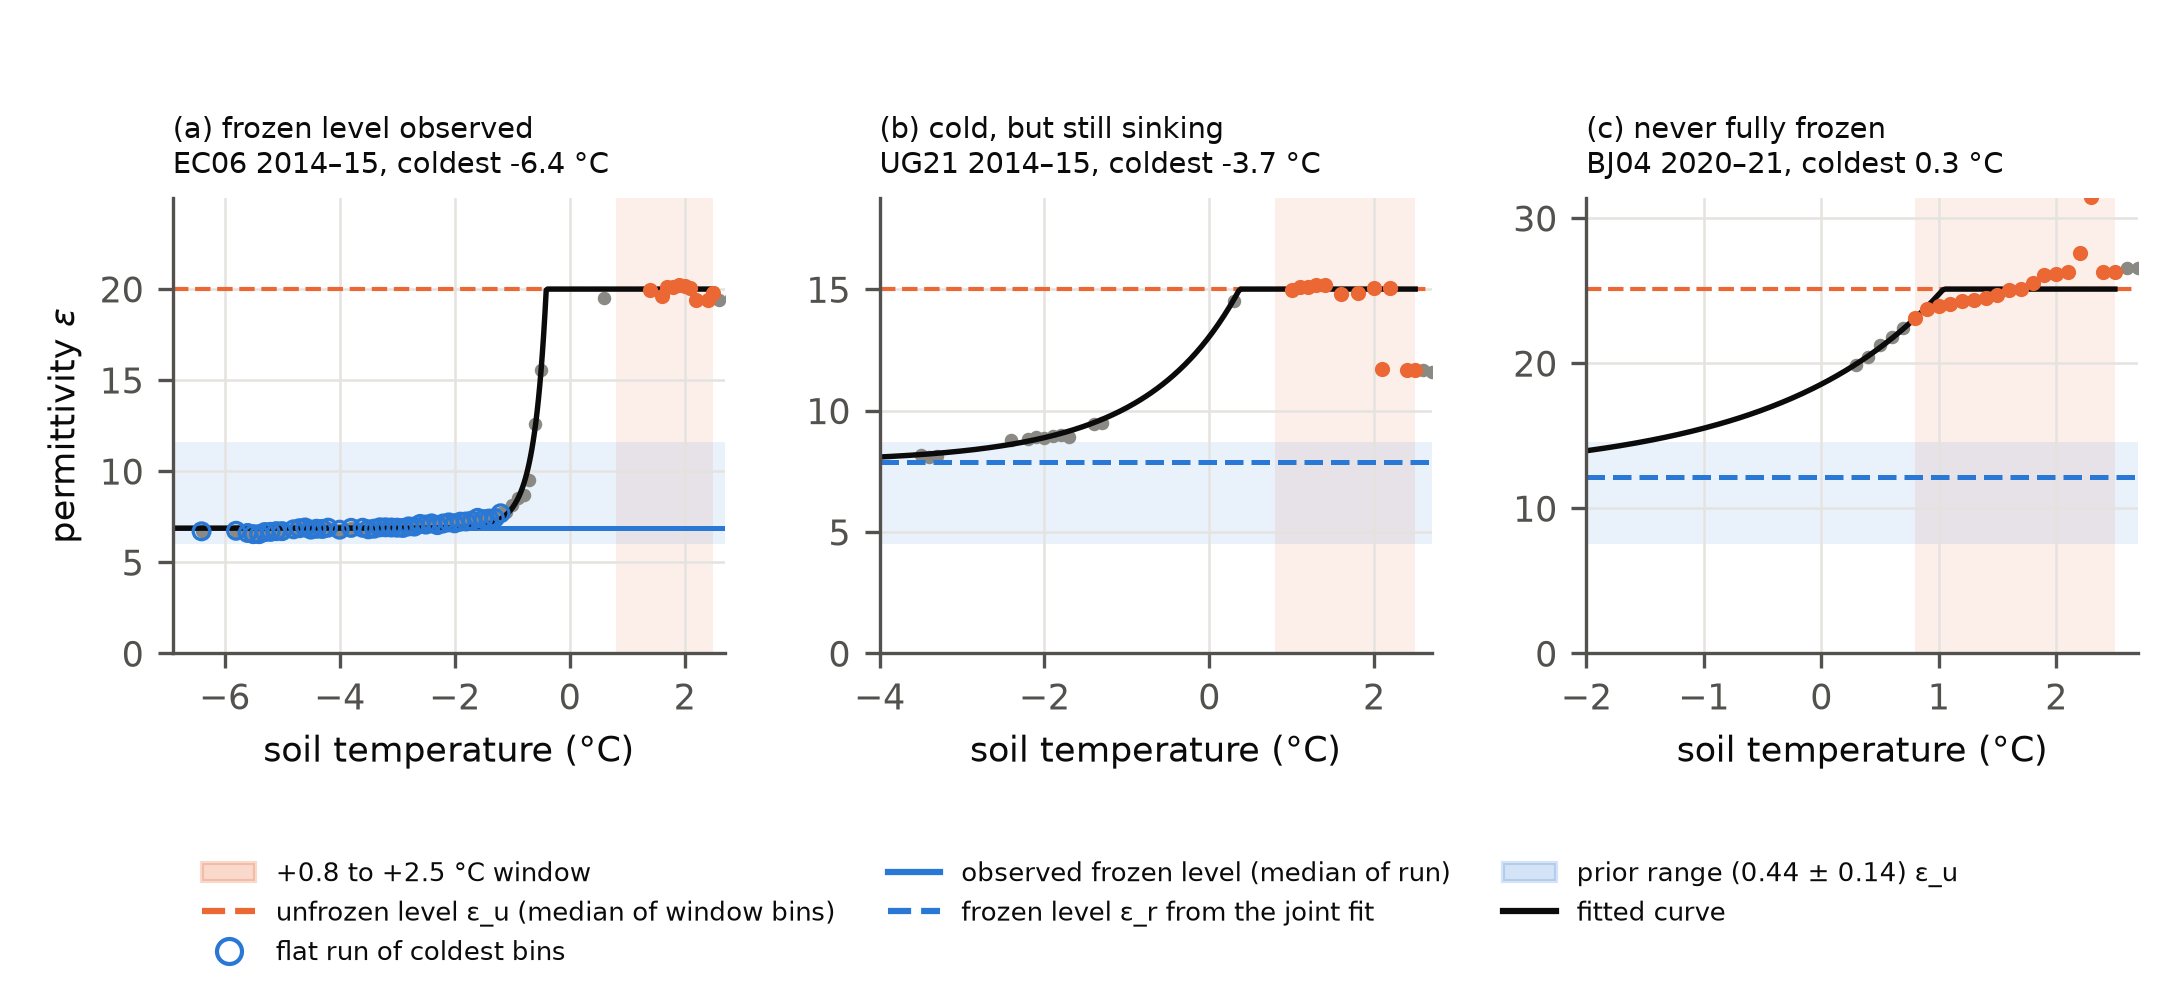
\includegraphics[width=\textwidth]{figures/fig_levels.png}
\caption{How the unfrozen and frozen levels are obtained, for three topsoil
winters at Kenaston (EC06, UG21) and James Bay (BJ04). Dots are 0.1\,$^{\circ}$C
bin medians of the freezing leg; orange dots fall in the $+0.8$ to
$+2.5$\,$^{\circ}$C window whose median is $\varepsilon_u$ (orange dashed line;
20.0, 15.0 and 25.1). The blue band is the prior range
$(0.44 \pm 0.14)\,\varepsilon_u$ and the blue dashed line the frozen level from
the joint fit. (a) The coldest bins form a flat run (open circles) whose
median, 6.9, is the observed frozen level; the fit reproduces it. (b) The soil
reached $-3.7$\,$^{\circ}$C but its permittivity was still decreasing; no
frozen level is observed and the fit places it at 7.9, just below the lowest
bin. (c) The soil never fell below $+0.3$\,$^{\circ}$C; the frozen level,
12.2, is set by the prior.}
\label{fig:levels}
\end{figure*}

\begin{figure*}[t]
\centering
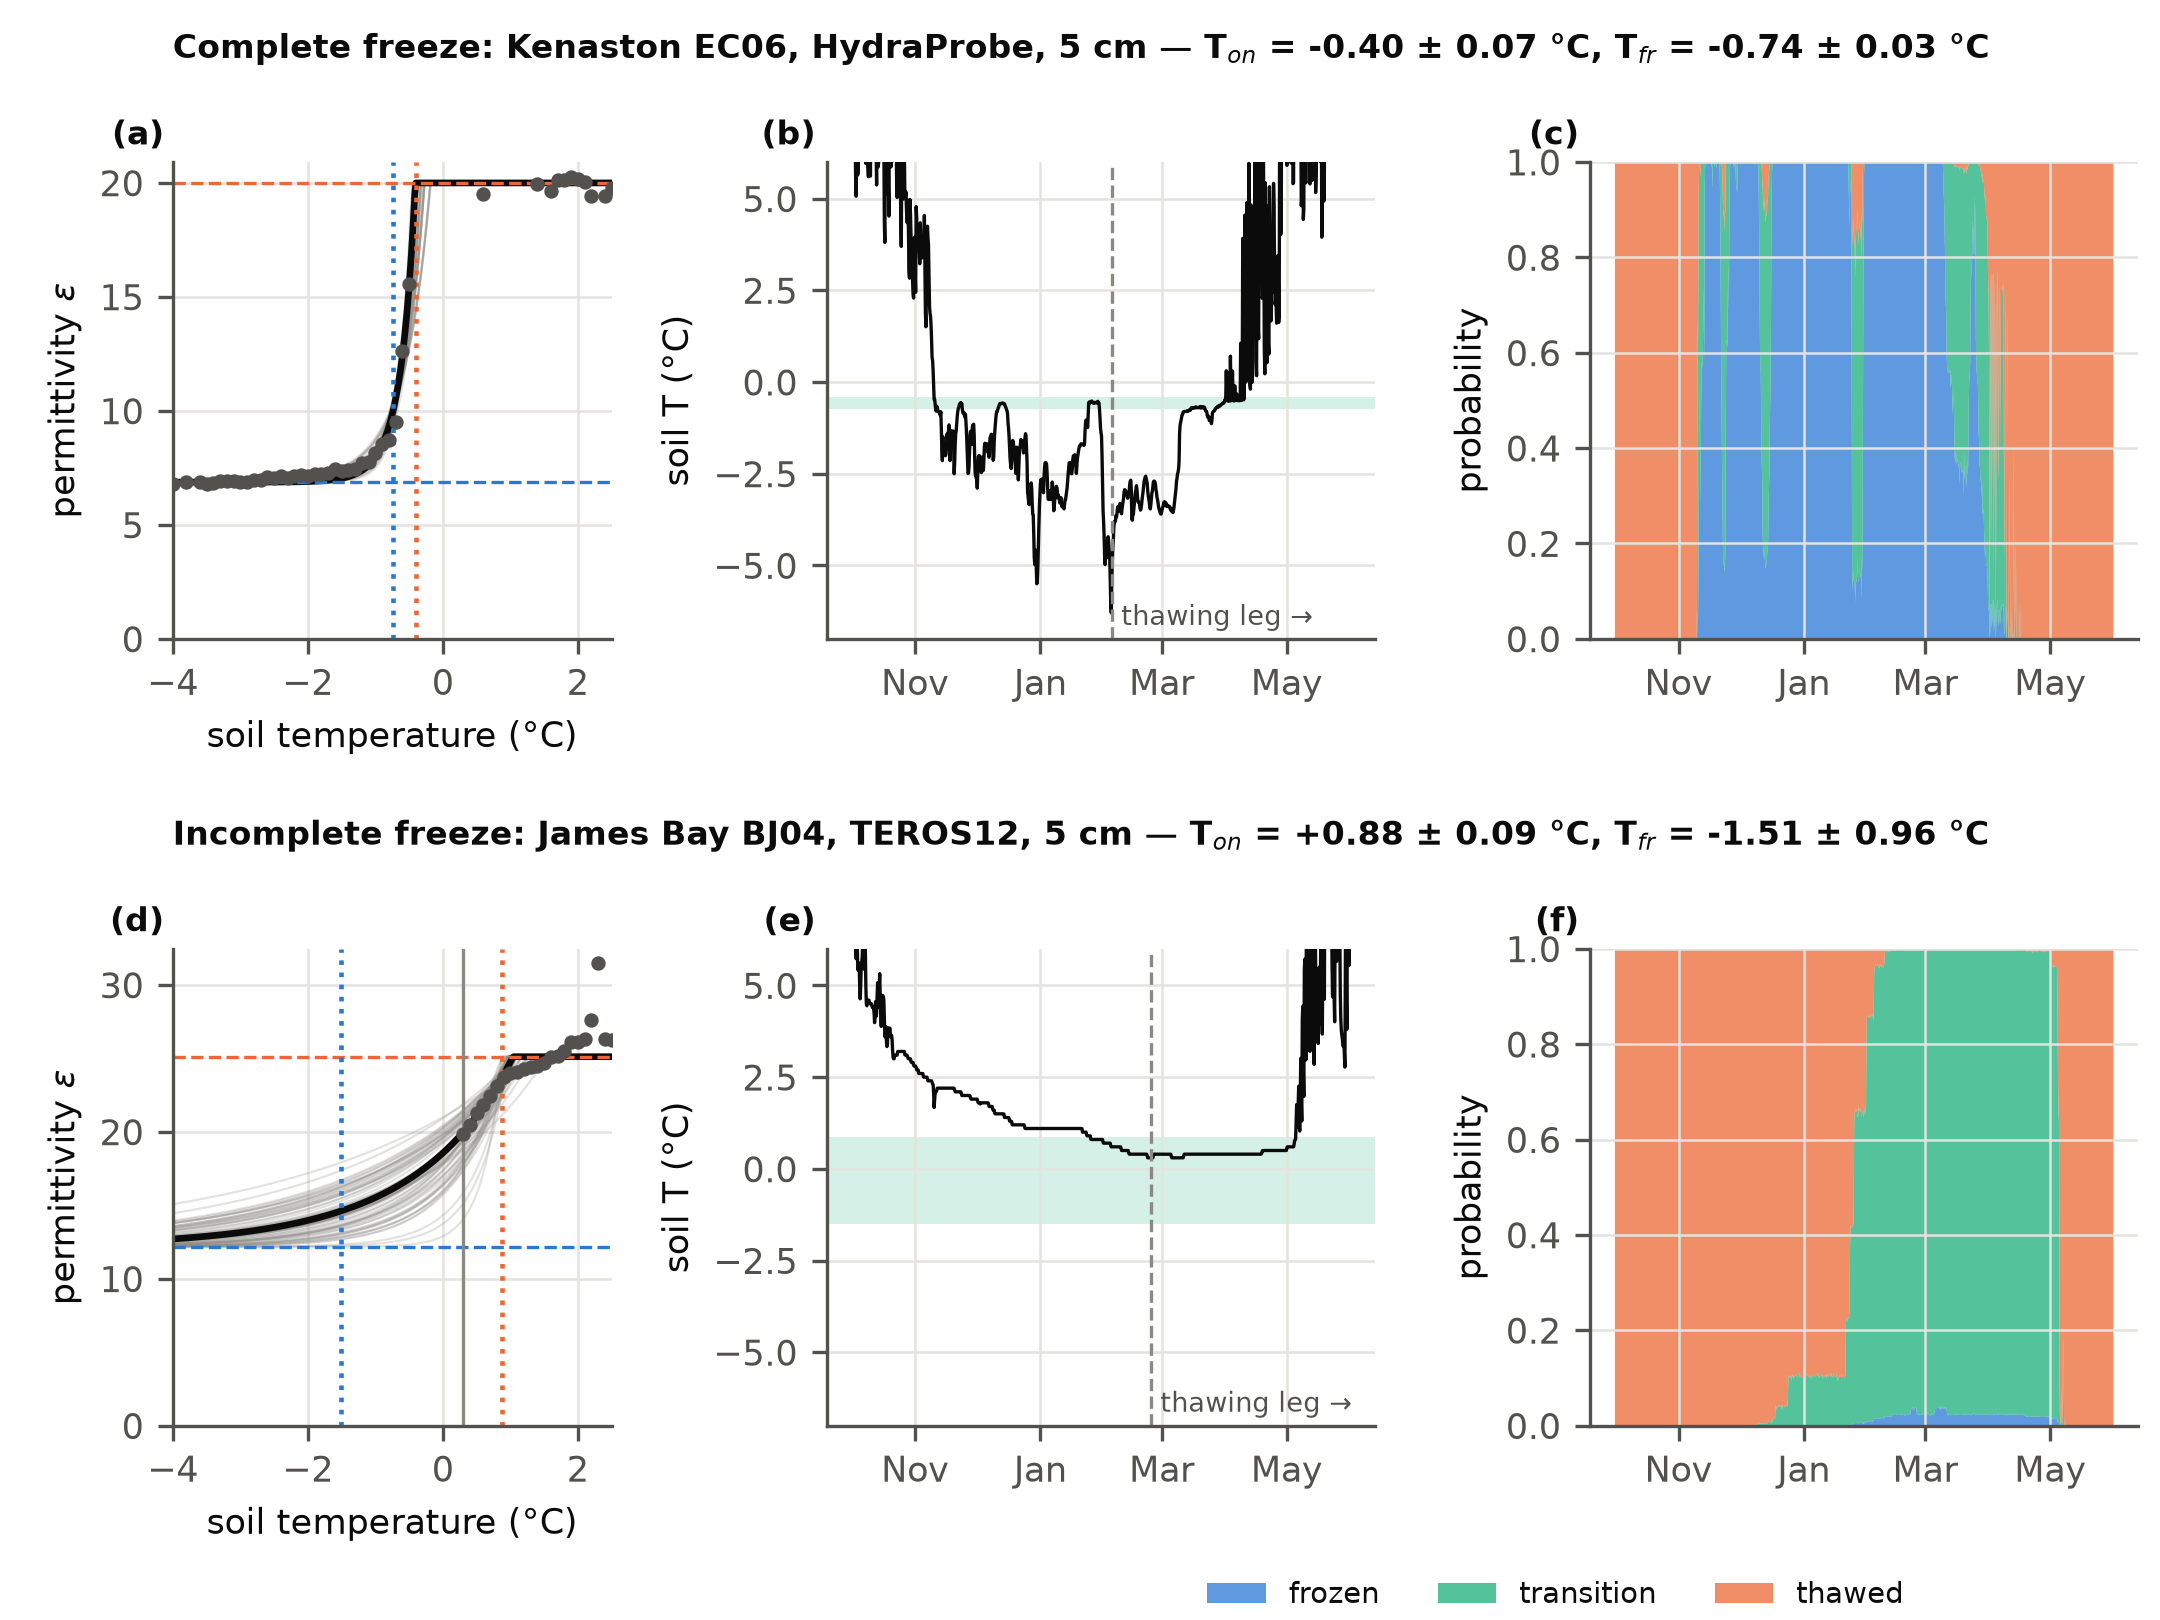
\includegraphics[width=\textwidth]{figures/fig_example_winters.png}
\caption{Two topsoil winters. (a, d) Binned permittivity against soil
temperature with the fitted curve (black), bootstrap curves (grey), unfrozen and
frozen levels (dashed), $T_{on}$ and $T_{fr}$ (dotted) and the coldest soil
temperature of the winter (grey line). (b, e) Soil temperature through the
freeze year with the transition range $T_{fr}$--$T_{on}$ (green) and the start
of the thawing leg. (c, f) Hourly state probabilities (6-hour means). In
(a--c) the soil freezes completely and the frozen level is observed; in (d--f)
the soil never falls below $+0.3$\,$^{\circ}$C, the frozen level relies on the
prior, and $T_{fr}$ is highly uncertain.}
\label{fig:example-winters}
\end{figure*}

\begin{figure}[t]
\centering
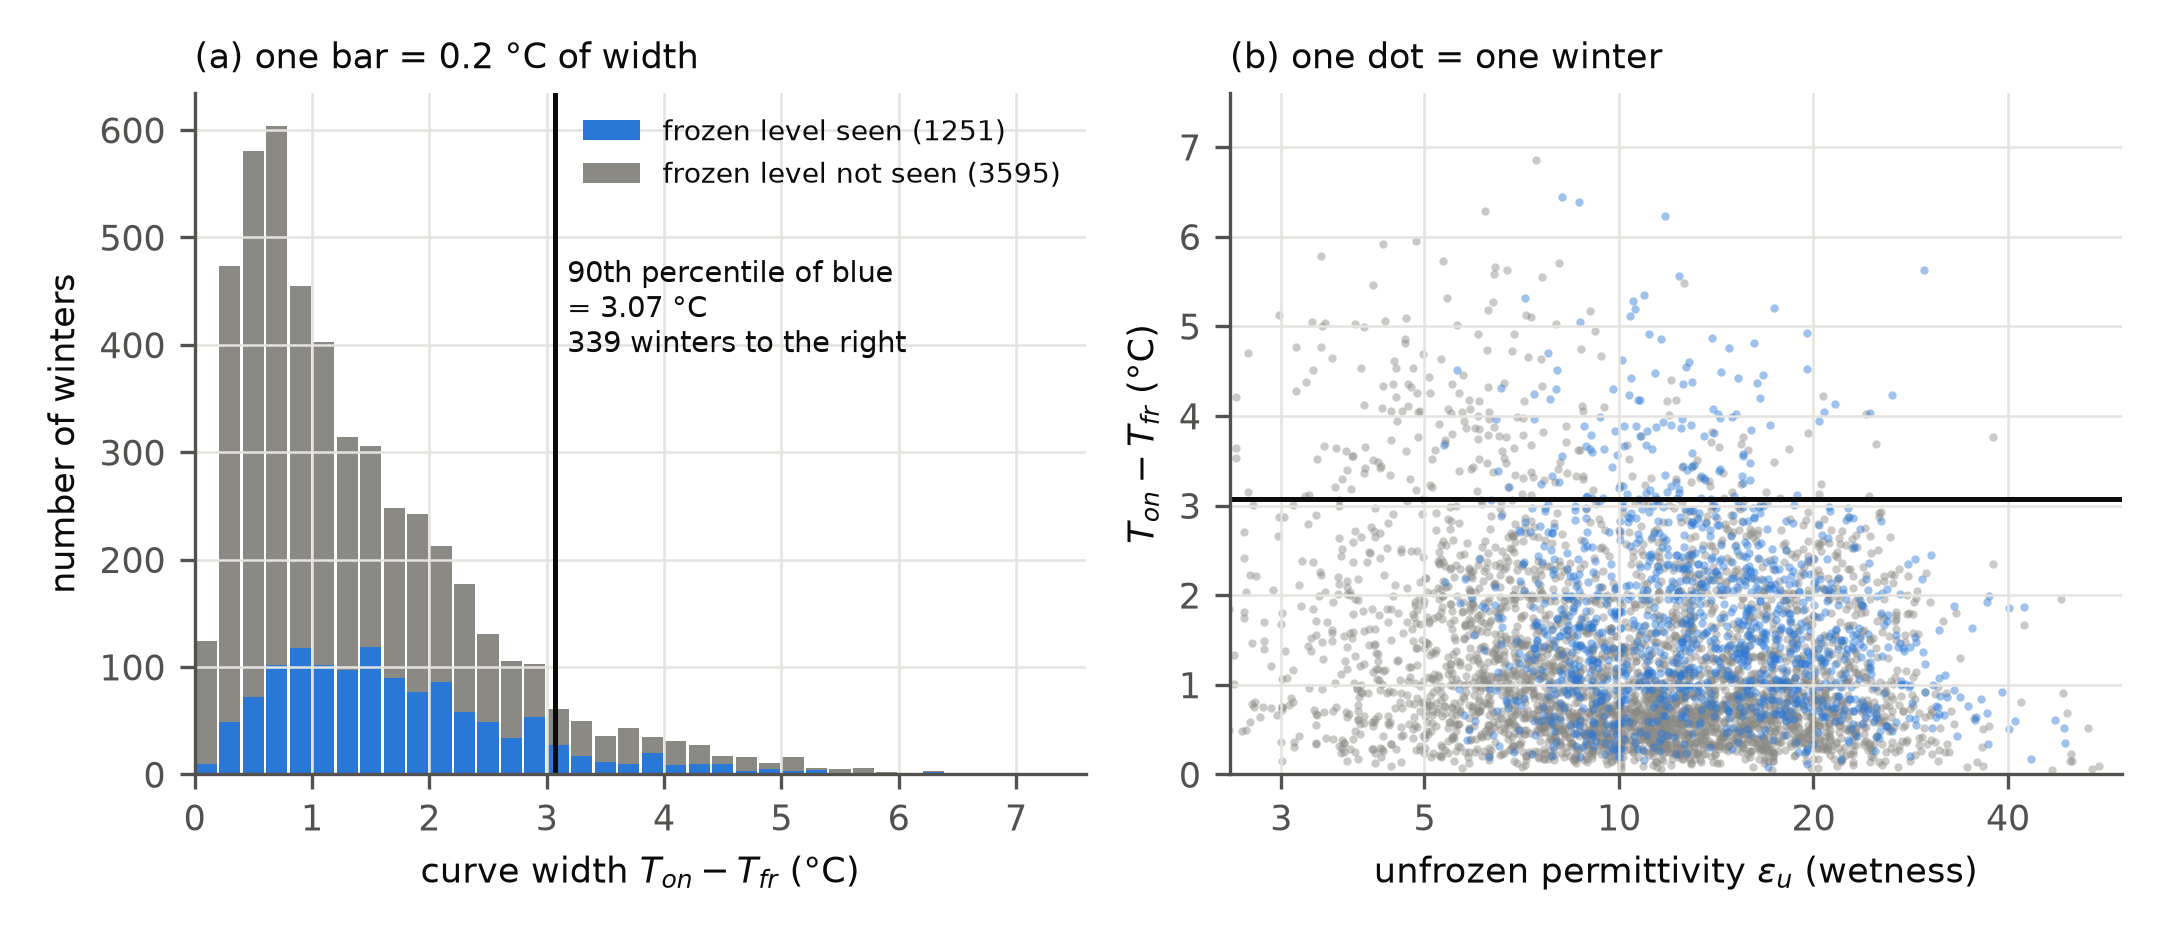
\includegraphics[width=\columnwidth]{figures/fig_widths.png}
\caption{Curve width $T_{on}-T_{fr}$ of 4,846 fitted topsoil winters. Blue:
winters whose frozen level is seen in the data (1,251); grey: all other fitted
winters. The black line is the 90th percentile of the blue winters
(3.07\,$^{\circ}$C); winters above it are treated as slow freezes. (a)
Histogram with 0.2\,$^{\circ}$C bars, stacked. (b) Width against the unfrozen
permittivity.}
\label{fig:widths}
\end{figure}

\begin{figure}[t]
\centering
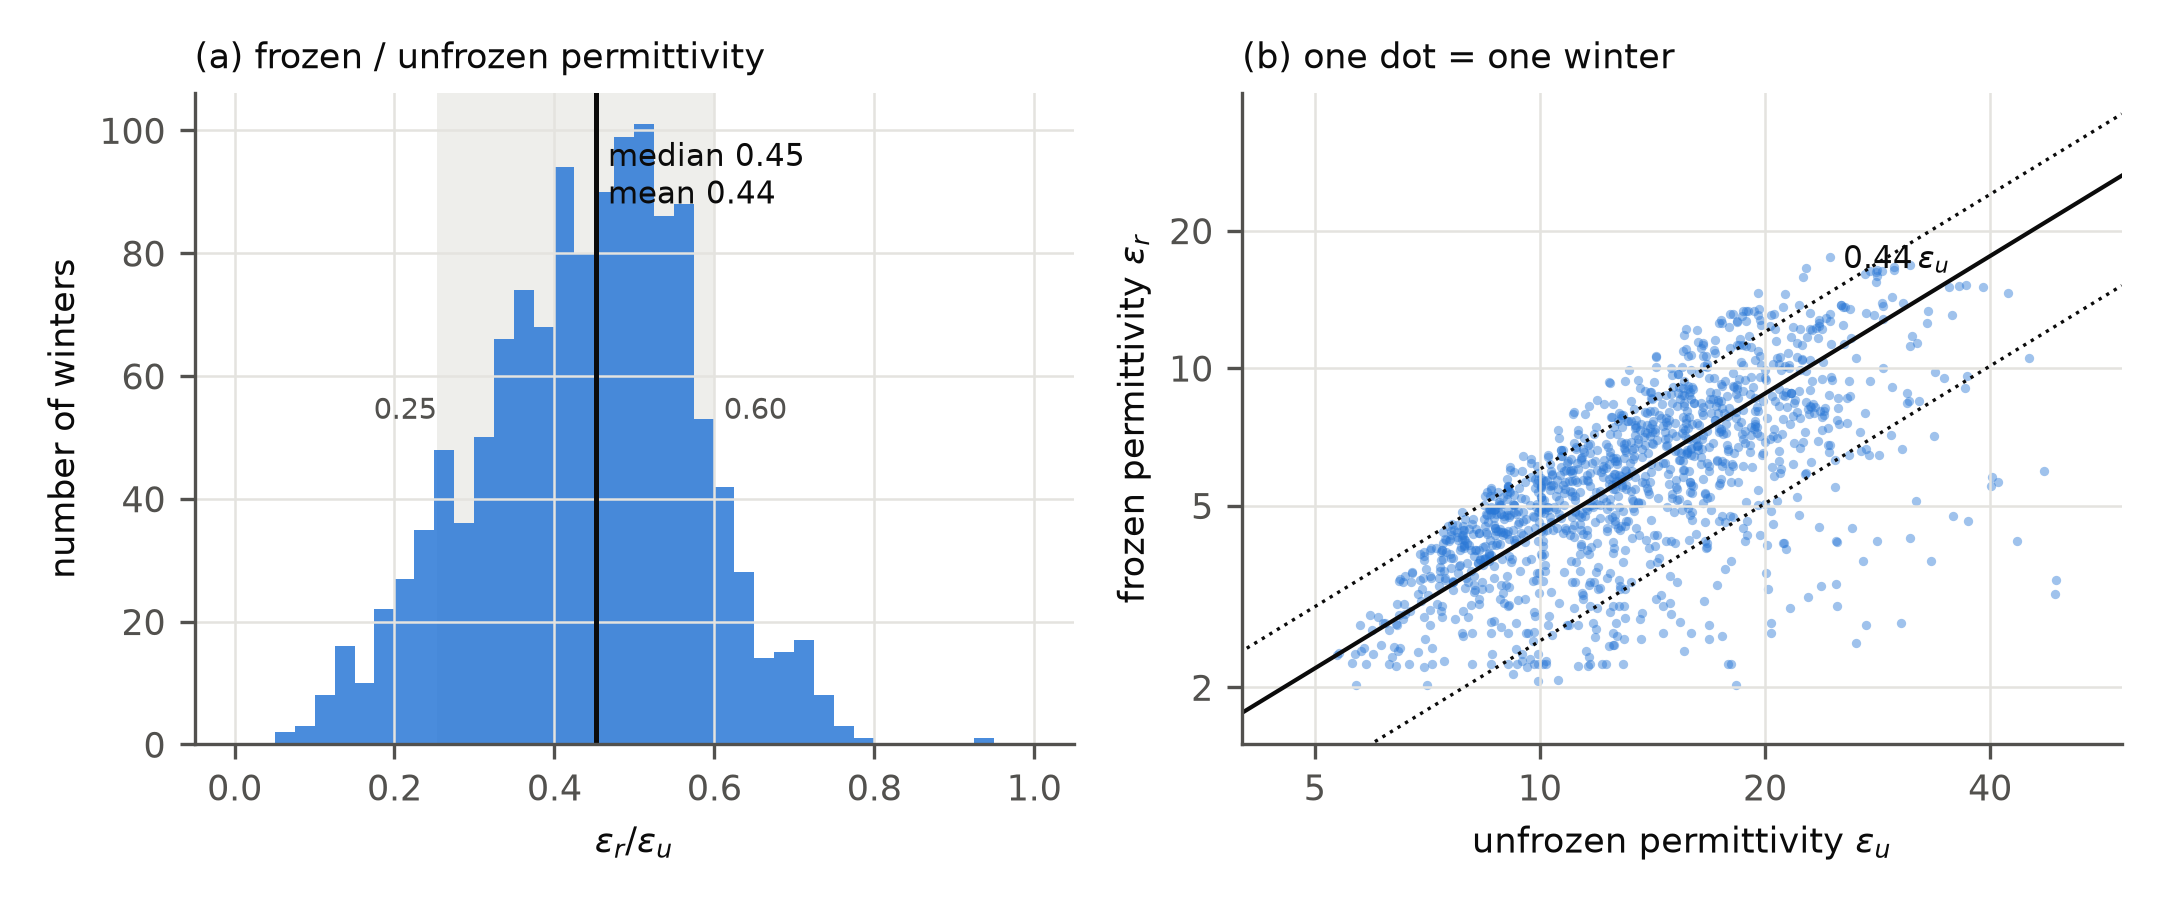
\includegraphics[width=\columnwidth]{figures/fig_frozen_fraction.png}
\caption{Frozen and unfrozen permittivity of 1,285 topsoil winters at 467 sensors
whose soil reached $-5$\,$^{\circ}$C with an observed frozen level. (a) Ratio
$\varepsilon_r/\varepsilon_u$ (grey band: 10th--90th percentile). (b) One dot
per winter; the solid line is $0.44\,\varepsilon_u$ and the dotted lines the
10th and 90th percentiles.}
\label{fig:frozen-fraction}
\end{figure}

\subsection{Sensors with soil temperature only}
\label{sec:state-temperature}
% Counts are estimates from the per-winter fits (scripts/winter_widths.py); update after the full run.
Without a moisture or permittivity record no curve can be fitted, so the
thresholds of these sensors are borrowed from fitted sensors. The same
applies to moisture sensors in years without an accepted fit (for example a
mild winter with less than 15\,\% of the expected drop). Of the 3,942 topsoil
sensors, about 1,430 have at least one fitted winter, about 790 have moisture
data but no fitted winter, and about 1,710 measure temperature only or have no
usable paired record.

Fitted winters are first pooled per sensor. Each winter's $T_{on}$ and
$T_{fr}$ are shrunk towards the sensor mean with a DerSimonian--Laird
random-effects model \citep{dersimonian1986}; the winter keeps its own
uncertainty, because errors in the frozen level are shared by all winters of
a sensor. Sensor means are combined into group means in the same way, and the
between-sensor spread is part of the uncertainty of each group mean. A
sensor-year without its own fit then uses the first available of
(1) the same sensor's other fitted winters, (2) sensors of the same network
with the same temperature-probe type, (3) sensors with the same probe type in
any network, (4) sensors of the same network with another probe type, (5)
sensors with the same RESOLVE biome and SoilGrids USDA texture class
(at least three sensors), and (6) all topsoil sensors. Groups never mix depth
classes. Level (1) competes with the first available of levels (2)--(6): the
one with the smaller combined uncertainty of $T_{on}$ and $T_{fr}$ is used,
because a sensor with only one or two fitted winters that disagree gives a
poorer estimate than its group.

The order follows two findings. First, fitted thresholds contain the
thermistor offset of each probe, so the probe type matters: at eight James Bay
sites where a TEROS12 and an iButton were co-located, the difference of their
zero-curtain temperatures was $+0.02 \pm 0.16$\,$^{\circ}$C. No offset
correction is applied, but levels (4)--(6), which may mix probe types, add
0.16\,$^{\circ}$C to the uncertainty of both thresholds. Second, the groupings
were ranked by how well they predict thresholds at a site whose own thresholds
are known but withheld (Fig.~\ref{fig:grouping}). The test uses the 4,507
fitted topsoil winters at 978 sites (slow freezes excluded). Each site in turn
is treated as if it had no moisture record: it is removed, every grouping
predicts its $T_{on}$ and $T_{fr}$ as the median of the other sites' winters in
the same group (at least three, otherwise the median of all), and the
prediction is compared with the site's own fitted values. Removing whole sites
rather than single winters prevents a sensor from being predicted by its
neighbours at the same site. For James Bay BJ04, for example, all other sites
give $T_{on} = +0.34$\,$^{\circ}$C, forest on sandy loam $+0.40$, boreal forest
on sandy loam $+0.58$ and the other James Bay TEROS12 sensors $+0.66$, against
a fitted $+0.87$\,$^{\circ}$C (Fig.~\ref{fig:grouping}a). Over all winters,
network and probe type gave the smallest median absolute error ($T_{on}$
0.24\,$^{\circ}$C, $T_{fr}$ 0.42\,$^{\circ}$C, against 0.32 and
0.51\,$^{\circ}$C without grouping). Among groupings by environment, biome and
texture class together did best (0.26 and 0.43\,$^{\circ}$C), ahead of land
cover and texture (0.27, 0.44) and of land cover alone (0.31, 0.49); adding
land cover to biome and texture did not improve it further and left more
sites without a group (Fig.~\ref{fig:grouping}b, c). Borrowed thresholds also receive
the extra 0.1\,$^{\circ}$C on $T_{on}$ and 0.5\,$^{\circ}$C on $T_{fr}$, and a
minimum standard deviation of 0.1\,$^{\circ}$C. From the current fits, about
89\,\% of the temperature-only topsoil sensors take their thresholds from a
network and probe match, 2\,\% from the probe type, 4\,\% from their network
with another probe type, 5\,\% from biome and texture, and fewer than
0.5\,\% from all sensors. Each hour reports the level used
(\texttt{threshold\_source}).

\begin{figure}[t]
\centering
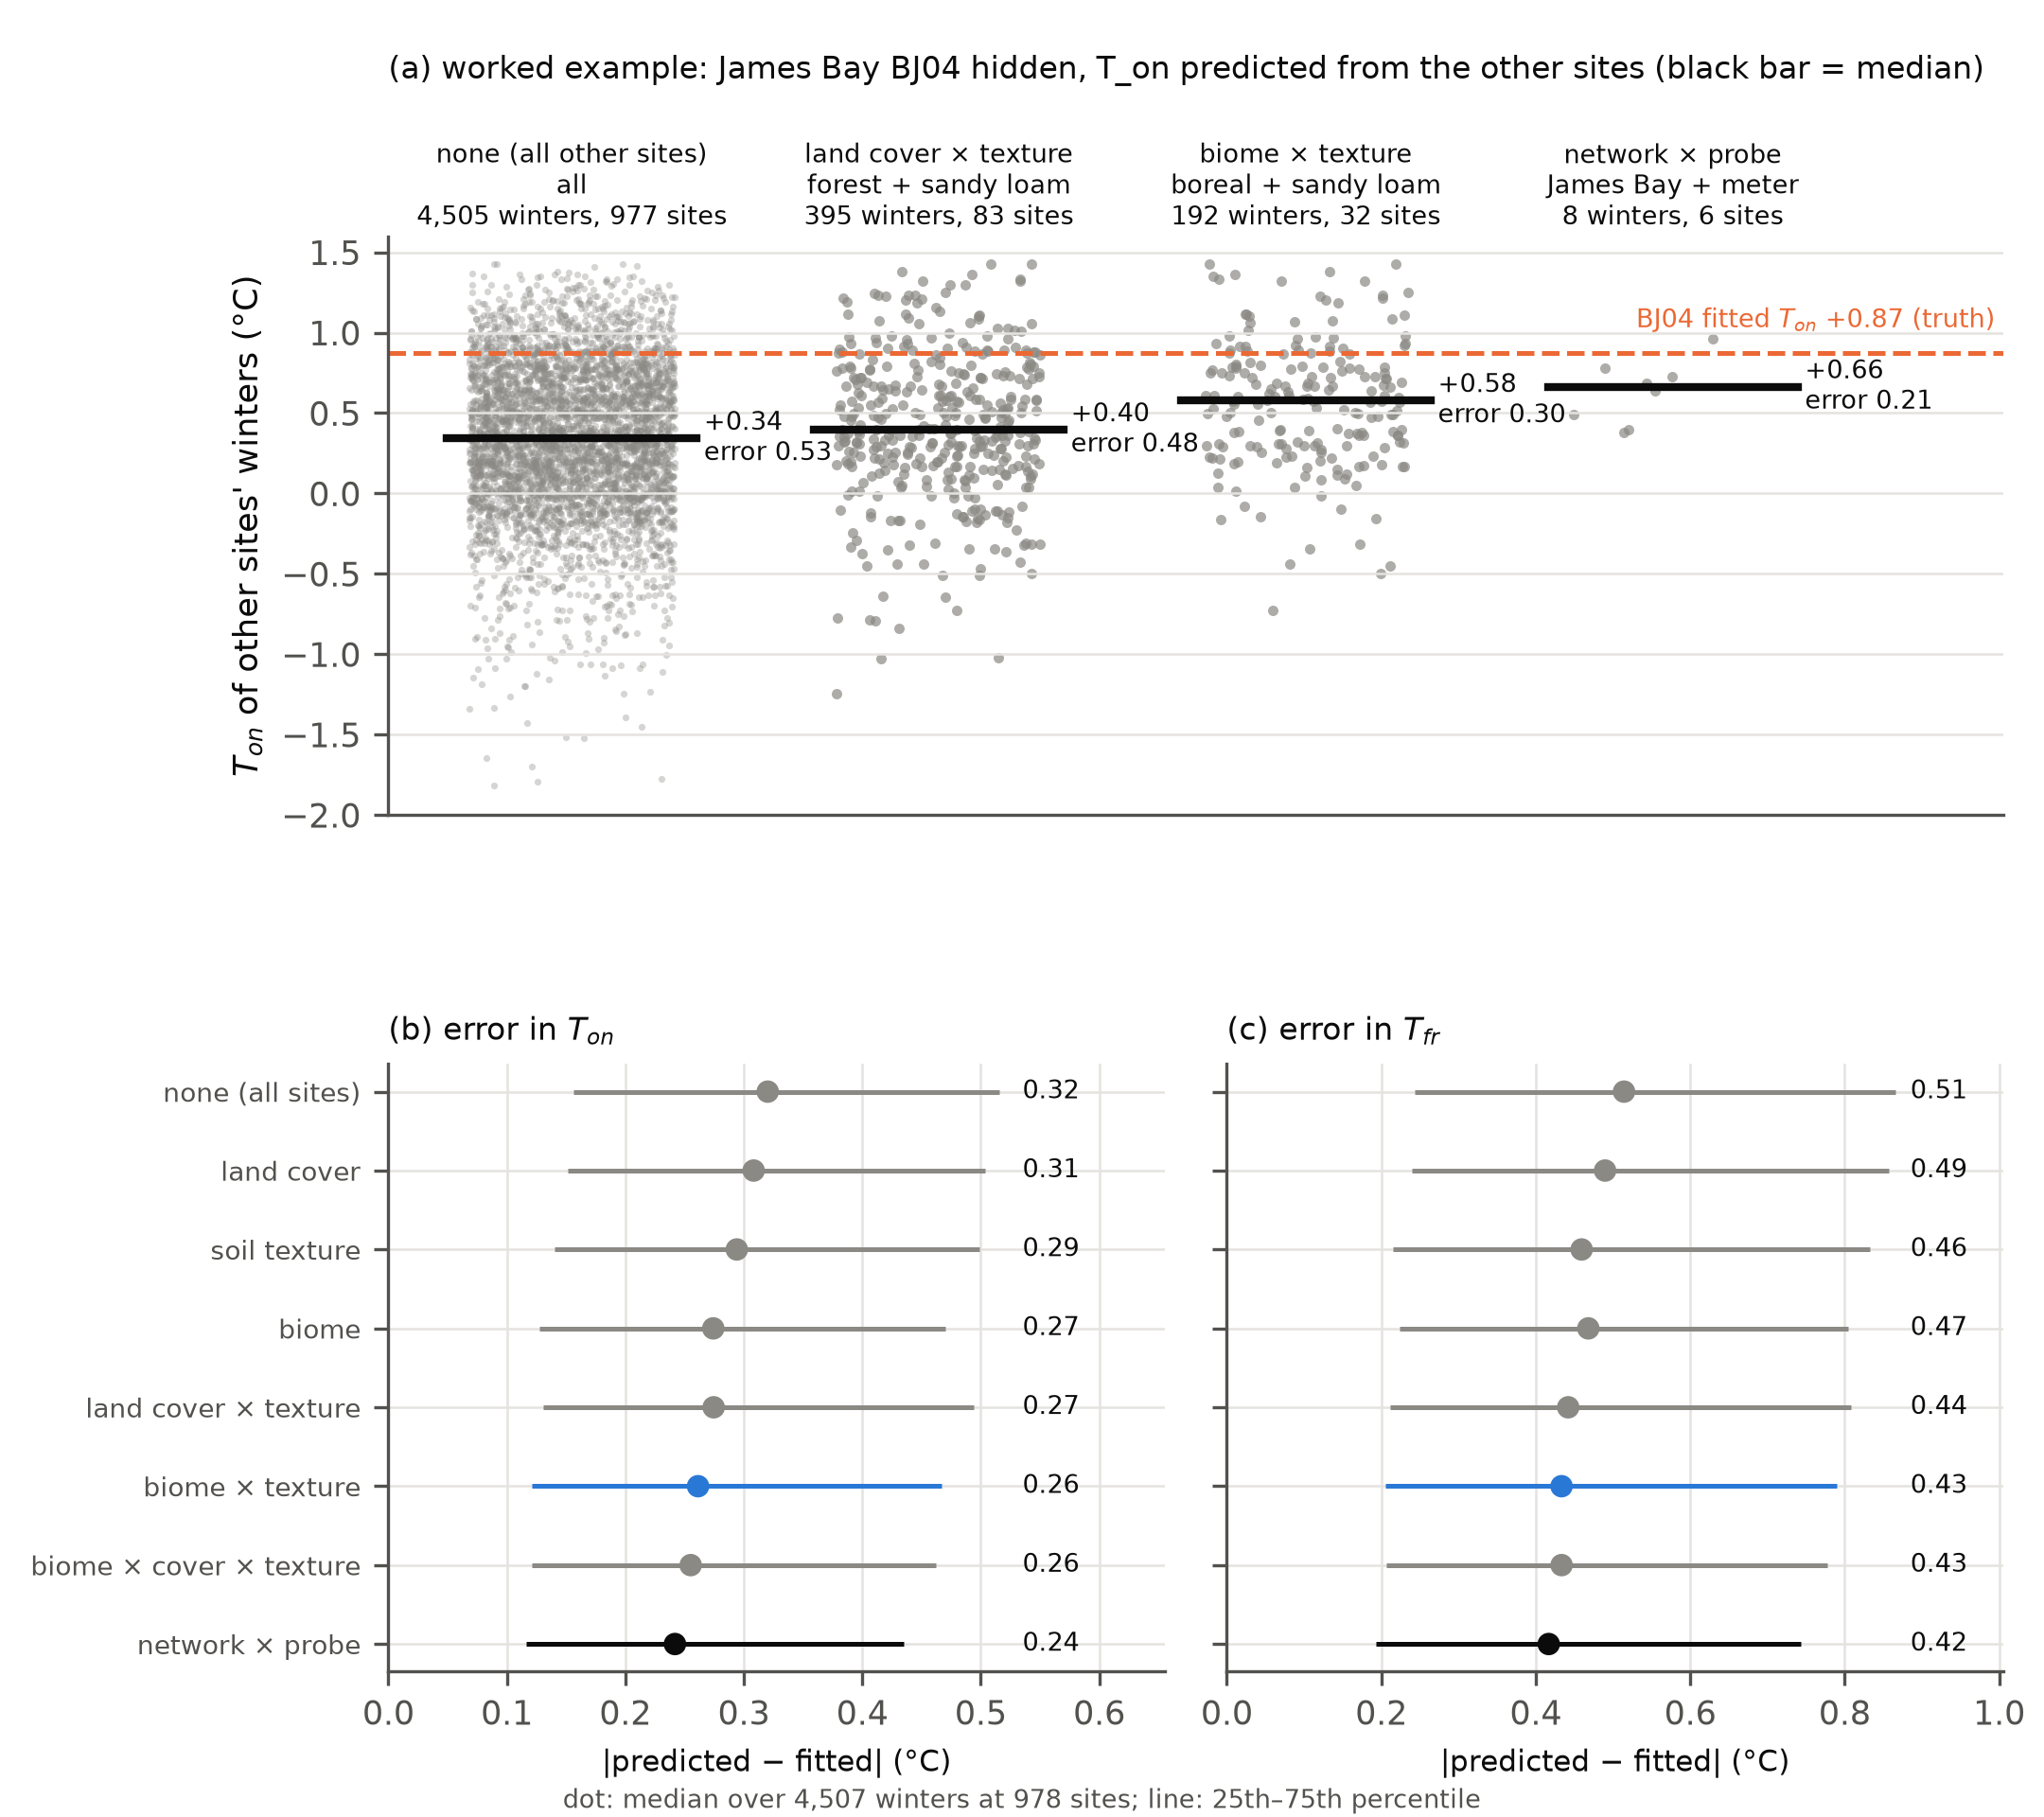
\includegraphics[width=\columnwidth]{figures/fig_grouping.png}
\caption{Choosing where sensors without a fit borrow their thresholds. Each
site with fitted winters is withheld in turn and its thresholds are predicted
from the other sites. (a) James Bay BJ04: grey dots are the fitted $T_{on}$ of
the other sites' winters in each candidate group, the black bar their median
(the prediction), the dashed line BJ04's own fitted $T_{on}$. (b, c) Absolute
prediction error of $T_{on}$ and $T_{fr}$ for each grouping over 4,507 topsoil
winters at 978 sites: dot, median; line, 25th--75th percentile. Blue: the
environment grouping used (level 5); black: network and probe type (level 2).}
\label{fig:grouping}
\end{figure}

\subsection{Hourly state probabilities and freeze dates}
\label{sec:state-hourly}
For every hour, 400 pairs $(T_{on},T_{fr})$ are drawn, from the winter's
bootstrap distribution rescaled to its final uncertainty or, for borrowed
thresholds, from normal distributions around the borrowed means. Each pair is
compared with the measured temperature perturbed by 0.1\,$^{\circ}$C
thermometer noise, and the probability of thawed, transitional and frozen soil
is the fraction of draws in each state; the mean of $F$ over the draws gives
the expected frozen fraction. Pairs with $T_{fr} \ge T_{on}$ are redrawn. The
thermistor offset of each probe is already contained in its thresholds, so
only the random thermometer error is added. Each hour is also assigned to the
freezing or thawing leg so that spring, when meltwater and thaw hysteresis
occur but the same thresholds are applied, can be analysed separately.

Each day with at least 75\,\% of the possible readings takes the most
frequent hourly label. Following \citet{rautiainen2025}, the freeze start is
the first day on or before 1~March that begins at least five consecutive
frozen days, and the transition onset the first day that begins five
consecutive days that are not thawed. The freeze end is the first day of the
thawing leg that begins five consecutive thawed days, reported for years with
a transition onset; \citet{rautiainen2025} define no spring date because wet
snow masks the soil at L-band, so this rule mirrors the autumn one. Because
thresholds use the whole freezing leg, the product is retrospective.

\section{Data quality, validation, and limitations}
An independent implementation recomputed grid cells, land-cover assignments,
representativeness flags, and SoilGrids values from source definitions and
rasters. Approximately 4.7 million comparisons showed no discrepancies in the
derived metadata. These checks verify the processing, not the accuracy of the
original sensor measurements. Source quality flags are retained where
available, but no additional measurement-level quality control was applied.
Some source time conventions are assumed, 332 AmeriFlux sensor depths are
inferred, and SoilGrids properties are model estimates rather than site
measurements. The uncertainty and plausibility assessment required for the
released data product still needs to be completed.

\conclusions
The collection brings hourly soil observations and spatial context into a
common format for freeze--thaw studies. Its final scope and claims depend on
the releasable data product and its independent quality assessment.

\codedataavailability{Processing code is available at
\url{https://github.com/hesam-salmabadi/sfcc-label}. The dataset described in
this draft is not yet deposited as a public, versioned release. Before ESSD
submission, provide a repository review link or DOI for the releasable data
product, cite each original source, and explain any records that cannot be
redistributed. ISMN observations cannot be redistributed under their source
terms and are available from \url{https://ismn.earth}; AmeriFlux source data
are available from \url{https://ameriflux.lbl.gov}.}

\authorcontribution{Author contributions to be confirmed with all co-authors.}
\competinginterests{Competing-interest declarations to be confirmed with all co-authors.}

\begin{acknowledgements}
Acknowledgements and funding to be completed with all co-authors.
\end{acknowledgements}

\begin{thebibliography}{}
\bibitem[Bai et al.(2018)]{bai2018}
Bai, R., Lai, Y., Zhang, M., and Yu, F.: Theory and application of a novel soil
freezing characteristic curve, Appl. Therm. Eng., 129, 1106--1114, 2018.

\bibitem[Cohen et al.(2021)]{cohen2021}
Cohen, J., Rautiainen, K., Lemmetyinen, J., Smolander, T., Vehvil\"ainen, J.,
and Pulliainen, J.: Sentinel-1 based soil freeze/thaw estimation in boreal
forest environments, Remote Sens. Environ., 254, 112267, 2021.

\bibitem[DerSimonian and Laird(1986)]{dersimonian1986}
DerSimonian, R. and Laird, N.: Meta-analysis in clinical trials, Control.
Clin. Trials, 7, 177--188, 1986.

\bibitem[Rautiainen et al.(2025)]{rautiainen2025}
Rautiainen, K., Holmberg, M., Cohen, J., Mialon, A., Schwank, M.,
Lemmetyinen, J., de la Fuente, A., and Kerr, Y.: An operational SMOS soil
freeze--thaw product, Earth Syst. Sci. Data, 17, 5337--5353,
https://doi.org/10.5194/essd-17-5337-2025, 2025.

\bibitem[Salmabadi et al.(2026)]{salmabadi2026}
Salmabadi, H., Pardo Lara, R., Berg, A., Mavrovic, A., Hanes, C., Montpetit, B.,
and Roy, A.: In situ monitoring of seasonally frozen ground using soil freezing
characteristic curve in permittivity--temperature space, The Cryosphere, 20,
1635--1654, 2026.

\bibitem[Topp et al.(1980)]{topp1980}
Topp, G. C., Davis, J. L., and Annan, A. P.: Electromagnetic determination of
soil water content: measurements in coaxial transmission lines, Water Resour.
Res., 16, 574--582, 1980.

\bibitem[Brodzik et al.(2012)]{brodzik2012}
Brodzik, M. J., Billingsley, B., Haran, T., Raup, B., and Savoie, M. H.:
EASE-Grid 2.0: Incremental but significant improvements for Earth-gridded data
sets, ISPRS Int. J. Geo-Inf., 1, 32--45, 2012.

\bibitem[Dinerstein et al.(2017)]{dinerstein2017}
Dinerstein, E., Olson, D., Joshi, A., Vynne, C., Burgess, N. D., Wikramanayake,
E., Hahn, N., Palminteri, S., Hedao, P., Noss, R., et al.: An ecoregion-based
approach to protecting half the terrestrial realm, BioScience, 67, 534--545,
https://doi.org/10.1093/biosci/bix014, 2017.

\bibitem[Poggio et al.(2021)]{poggio2021}
Poggio, L., de Sousa, L. M., Batjes, N. H., Heuvelink, G. B. M., Kempen, B.,
Ribeiro, E., and Rossiter, D.: SoilGrids 2.0: producing soil information for
the globe with quantified spatial uncertainty, SOIL, 7, 217--240, 2021.
\end{thebibliography}

\end{document}
